\chapter{Lecture 5: New Revolutions in Particle Physics: Basic Concepts}

These notes follow Leonard Susskind's fifth lecture in \emph{Particle Physics 1: Basic Concepts}, in a format curated by LazyingArt LLC. The lecture begins with a question about wave motion, not with fermions, and that is already the point: before we can talk sensibly about particles, creation operators, and antiparticles, we must separate what is physically measurable from what is merely a formal feature of the way we write a wave. From there the lecture moves through symmetry and conservation laws, turns to the algebra of fermions, and closes by showing how the many-body idea of a hole points toward Dirac's idea of the antiparticle.

\section{Phase Velocity and What Is Actually Measured}

The opening question is about phase velocity and group velocity. Susskind's answer begins from the simplest possible wave. Let us write
\begin{equation}
\psi(x,t)=e^{i(kx-\omega t)},
\end{equation}
or, if we prefer a real wave,
\begin{equation}
\psi(x,t)=\sin(kx-\omega t).
\end{equation}
A crest, or more generally any point of fixed phase, moves so that
\begin{equation}
kx-\omega t=\text{const.}
\end{equation}
Therefore
\begin{equation}
x=\frac{\omega}{k}t,
\qquad
v_{\mathrm{phase}}=\frac{\omega}{k}=\frac{\lambda}{T}.
\end{equation}
So the phase velocity is simply the speed with which constant phase travels.

For a nonrelativistic Schr\"odinger wave, after correcting the spoken slip in the lecture, the dispersion relation is
\begin{equation}
\omega=\frac{k^2}{2m}.
\end{equation}
Hence
\begin{equation}
v_{\mathrm{phase}}=\frac{\omega}{k}=\frac{k}{2m}.
\end{equation}
But the classical velocity of a particle of momentum \(p=k\) is \(p/m=k/m\). There is an extra factor of two. This is the first sign that the phase velocity is not yet the thing we want to identify with the motion of the particle.

\subsection{Question \& Answer}

\paragraph{Question.} Why can changing \(\omega\) by a constant alter the phase velocity without changing the physics?

\paragraph{Answer.} This is the crucial destabilizing step in the lecture. Write the Schr\"odinger field schematically as
\begin{equation}
\psi(x,t)=\sum_k c_k\,e^{ikx}e^{-i\omega(k)t},
\end{equation}
where we suppress normalization factors, exactly as the lecture does. Now shift every frequency by the same constant:
\begin{equation}
\omega(k)\longrightarrow \omega(k)+c.
\end{equation}
Then every term in the sum picks up the same extra factor,
\begin{equation}
\psi(x,t)\longrightarrow e^{-ict}\psi(x,t).
\end{equation}
All observables of ordinary Schr\"odinger theory are built from \(\psi\) together with its complex conjugate. In particular,
\begin{equation}
\psi(x,t)\psi^\ast(x,t)\longrightarrow e^{-ict}e^{ict}\,\psi(x,t)\psi^\ast(x,t)=\psi(x,t)\psi^\ast(x,t).
\end{equation}
So the physics is unchanged. But the phase velocity would become
\begin{equation}
v_{\mathrm{phase}}\longrightarrow \frac{\omega+c}{k}=v_{\mathrm{phase}}+\frac{c}{k}.
\end{equation}
Therefore the phase velocity, at least in this context, cannot be the directly measurable propagation speed. It depends on a convention that does not affect observables.

\section{Wave Packets and the Velocity of Constructive Interference}

The lecture next asks what \emph{is} physically meaningful. The answer is the motion of a wave packet, that is, the motion of a localized lump built from many plane waves. The localization comes from interference: waves add in one region and cancel elsewhere.

To see this in the leanest possible way, Susskind takes two nearby waves,
\begin{equation}
\psi(x,t)=\sin(kx-\omega t)+\sin(k'x-\omega' t),
\end{equation}
with \(k'\) close to \(k\), and \(\omega'=\omega(k')\). The place where they reinforce each other most strongly is the place where their phases agree:
\begin{equation}
kx-\omega t=k'x-\omega' t.
\end{equation}
Rearranging,
\begin{equation}
(k-k')x=(\omega-\omega')t.
\end{equation}
Hence the locus of constructive interference moves according to
\begin{equation}
x=\frac{\omega-\omega'}{k-k'}\,t.
\end{equation}
When \(k'\) is very close to \(k\), this becomes
\begin{equation}
x=\frac{d\omega}{dk}\,t,
\qquad
v_{\mathrm{group}}=\frac{d\omega}{dk}.
\end{equation}
This is the group velocity: the speed of the reinforcing envelope, not of the individual phase crests.

Now return to the nonrelativistic dispersion relation, but keep the additive constant that the lecture used to expose the difference between the two velocities:
\begin{equation}
\omega=\frac{k^2}{2m}+c.
\end{equation}
Then
\begin{equation}
v_{\mathrm{group}}=\frac{d\omega}{dk}=\frac{k}{m}.
\end{equation}
Two things happen at once. First, the additive constant disappears. Second, the answer is exactly the classical particle velocity. This is why Susskind insists that it is the group velocity, not the phase velocity, that is tied to signals, particles, and actual propagation.

\section{Relativistic Dispersion and the Superluminal Puzzle}

Once the group velocity has emerged in this way, the lecture turns to the familiar anxiety about superluminal phase motion. For a relativistic particle,
\begin{equation}
E=\sqrt{p^2+m^2},
\qquad
\omega=\sqrt{k^2+m^2},
\qquad
\hbar=c=1.
\end{equation}
The phase velocity is then
\begin{equation}
v_{\mathrm{phase}}=\frac{\omega}{k}
=
\sqrt{\frac{k^2+m^2}{k^2}},
\end{equation}
which is greater than \(1\) whenever \(m\neq 0\). That is the moment in the lecture where one is invited to get a little nervous.

But the group velocity is
\begin{equation}
v_{\mathrm{group}}=\frac{d\omega}{dk}
=
\frac{k}{\sqrt{k^2+m^2}}
=
\sqrt{\frac{k^2}{k^2+m^2}},
\end{equation}
which is always less than \(1\). In this particular example,
\begin{equation}
v_{\mathrm{phase}}v_{\mathrm{group}}=1.
\end{equation}
Susskind explicitly remarks that this inverse relation is a special feature of the square-root dispersion relation; it is not a universal theorem.

When \(\omega\) is proportional to \(k\), all components move with the same speed and a wave packet does not spread. When \(\omega\) is a nonlinear function of \(k\), different Fourier components move differently, and the packet changes shape. This is the physical content of dispersion.

\begin{figure}
\centering

\includegraphics[width=0.72\textwidth]{lecture_05_figure_03.png}
\caption{Board evidence for the comparison between \(\omega/k\) and \(d\omega/dk\), together with the nonrelativistic dispersion \(\omega=k^2/(2m)+c\), the relativistic square-root relation, and the choice \(\hbar=c=1\).}
\end{figure}

For a massless particle, \(\omega=|k|\), and in one chosen branch one has simply \(\omega=k\), so both the phase and group velocities are equal to \(1\). In that linear case there is no dispersion. That is the clean limit against which the more general case is judged.

\section{Translation Symmetry, Phase Symmetry, and Conservation Laws}

Before getting to fermions, the lecture deliberately pauses for a recap of how symmetry shows up in amplitudes. The presentation is not a formal Noether-theorem digression. It stays very close to the field-theory bookkeeping already used earlier.

Suppose the time dependence of an amplitude has been reduced to a single exponential factor of the form
\begin{equation}
\mathcal{A}(t)\propto
\exp\!\left[
i\left(
\sum \omega_{\mathrm{out}}-\sum \omega_{\mathrm{in}}
\right)t
\right].
\end{equation}
If the process can happen with equal amplitude at any time, we integrate over all time and obtain
\begin{equation}
\int dt\,\mathcal{A}(t)\propto
\delta\!\left(
\sum \omega_{\mathrm{out}}-\sum \omega_{\mathrm{in}}
\right).
\end{equation}
That is the lecture's compact demonstration of energy conservation from time-translation invariance.

Momentum conservation is the same argument, but with space replacing time. If the process can occur with equal amplitude at any point in space, the position dependence takes the form
\begin{equation}
\mathcal{A}(x)\propto
\exp\!\left[
i\left(
\sum k_{\mathrm{in}}-\sum k_{\mathrm{out}}
\right)x
\right].
\end{equation}
Integrating over all space gives
\begin{equation}
\int dx\,\mathcal{A}(x)\propto
\delta\!\left(
\sum k_{\mathrm{out}}-\sum k_{\mathrm{in}}
\right),
\end{equation}
which is momentum conservation.

There is a third symmetry in the lecture, the overall phase rotation
\begin{equation}
\psi\longrightarrow e^{i\lambda}\psi.
\end{equation}
If an amplitude contains the same number of \(\psi\)'s and \(\psi^\dagger\)'s, this transformation does nothing. For a charge-carrying field, Susskind wants us to read that invariance as charge conservation. In the lecture the example in mind is the electron field: if the field carries electric charge, then invariance under a global phase change goes hand in hand with the statement that the net charge is conserved.

\section{Fermions, Anticommutators, and the Meaning of Exclusion}

Only after this recap does the lecture move to its main target. Bosons can pile into one state, and in fact they like to. Fermions do not merely dislike that arrangement; they forbid it. The Pauli principle is the physics, and the algebra is the bookkeeping that captures it.

Susskind writes the fermion field in the same spirit as the bosonic field,
\begin{equation}
\psi(x)=\sum_k c_k\,e^{ikx},
\qquad
\psi^\dagger(x)=\sum_k c_k^\dagger\,e^{-ikx},
\end{equation}
again suppressing normalization factors that were never the point of the lecture. The difference is not in the formal expansion; it is in the algebra of the operators.

To build that algebra, the lecture zooms all the way in to a single state. There are only two possibilities: the state is empty or occupied. Write those basis states as \(|0\rangle\) and \(|1\rangle\). Then the creation and annihilation operators act by
\begin{align}
c^\dagger |0\rangle &= |1\rangle,
&
c^\dagger |1\rangle &= 0,
\\
c|0\rangle &= 0,
&
c|1\rangle &= |0\rangle.
\end{align}
Here the symbol \(0\) on the right-hand side means the zero vector, not the vacuum state \(|0\rangle\). Susskind makes that distinction explicitly in the lecture because the algebra makes no sense if one confuses them.

Now act with \(c^\dagger c+cc^\dagger\) on the two allowed states. On \(|0\rangle\), the first term vanishes and the second returns \(|0\rangle\). On \(|1\rangle\), the second vanishes and the first returns \(|1\rangle\). Therefore
\begin{equation}
\{c,c^\dagger\}=cc^\dagger+c^\dagger c=1.
\end{equation}
Likewise, trying to create twice in the same state or annihilate twice in the same state always gives zero, so
\begin{equation}
\{c,c\}=0,
\qquad
\{c^\dagger,c^\dagger\}=0.
\end{equation}
For momentum-labelled fermions, the lecture generalizes this to
\begin{equation}
\{c_k,c_{k'}^\dagger\}=\delta_{kk'},
\qquad
\{c_k,c_{k'}\}=0,
\qquad
\{c_k^\dagger,c_{k'}^\dagger\}=0.
\end{equation}
This is the fermionic analog of the bosonic commutator algebra, with commutators replaced by anticommutators.

The lecture then sharpens the point. It is not enough to say that two fermions cannot have the same momentum. We should ask whether they can be created at the same place. At \(x=0\), the position-space creation operator gives
\begin{align}
\psi^\dagger(0)\psi^\dagger(0)|0\rangle
&=
\sum_{k,k'} c_k^\dagger c_{k'}^\dagger |0\rangle
\\
&=
\frac12
\sum_{k,k'}
\left(
c_k^\dagger c_{k'}^\dagger + c_{k'}^\dagger c_k^\dagger
\right)|0\rangle
\\
&=
\frac12
\sum_{k,k'}
\{c_k^\dagger,c_{k'}^\dagger\}|0\rangle
=0.
\end{align}
So the exclusion principle is not merely a statement about momentum eigenstates. It forbids putting two identical fermions into the same one-particle state, however we choose to represent that state.

\begin{figure}
\centering

\includegraphics[width=0.74\textwidth]{lecture_05_figure_04.png}

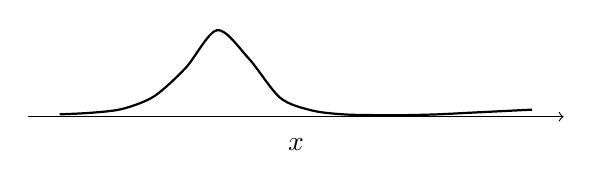
\begin{tikzpicture}[scale=1.0]
\draw[->] (-3.4,0) -- (3.4,0);
\draw[thick, smooth] plot coordinates {
(-3.0,0.03) (-2.6,0.05) (-2.2,0.10) (-1.8,0.26)
(-1.4,0.62) (-1.0,1.10) (-0.6,0.74) (-0.2,0.24)
(0.2,0.08) (0.6,0.03) (1.0,0.02) (1.4,0.02)
(1.8,0.03) (2.2,0.05) (2.6,0.07) (3.0,0.09)
};
\node at (0,-0.35) {$x$};
\end{tikzpicture}

\caption{The lecture's bridge from operator language to one-particle states: a localized wavefunction sketch on the board, beside the creation-operator expressions that enforce fermionic exclusion. The curve is redrawn for clarity while the screenshot preserves the original board layout.}
\end{figure}

\subsection{Question \& Answer}

\paragraph{Question.} What do we really mean by the same quantum state?

\paragraph{Answer.} This is where the lecture refuses to leave the Pauli principle in a crude form. A state is not, in general, specified by momentum alone. It may also involve spin; in an atom it involves an orbital wavefunction; in a beam it may be a localized packet. The correct statement is not ``same momentum'' but ``same quantum state.''

Susskind makes this concrete with widely separated locations. Let \(|N\rangle\) be a one-electron state localized in Nevada and \(|C\rangle\) one localized in Connecticut. Then
\begin{equation}
|+\rangle=\frac{1}{\sqrt{2}}\bigl(|N\rangle+|C\rangle\bigr),
\qquad
|-\rangle=\frac{1}{\sqrt{2}}\bigl(|N\rangle-|C\rangle\bigr)
\end{equation}
are two distinct one-particle states. One electron may occupy \(|+\rangle\) and another may occupy \(|-\rangle\), because these are different states. What one cannot do is put two electrons into the same state \(|+\rangle\).

This is also why the question ``Can two electrons have the same position but different momentum?'' is badly posed. Position and momentum do not commute, so one cannot specify both sharply. A localized packet may have a reasonably well-defined average momentum, but if the momentum is made infinitely sharp the localization is lost. The lecture insists on that point because it is exactly here that casual language about ``same momentum'' leads one astray.

\section{Bosons, Fermi Spheres, and Hole Excitations}

The next move is many-body physics in a finite box. If the available spatial volume is finite, the allowed momenta are discrete; in one dimension with periodic boundary conditions,
\begin{equation}
k=\frac{2\pi n}{L}.
\end{equation}
In three dimensions the allowed momentum vectors form a lattice in momentum space.

For bosons the ground state is immediate. Since the one-particle energy is
\begin{equation}
E=\frac{k^2}{2m},
\end{equation}
the lowest-energy state is \(k=0\), and all bosons can occupy it. The many-boson ground state is therefore a condensate at zero momentum.

For fermions, the first particle also goes into the lowest-energy state. But the next one cannot go there, and neither can the next after that. To keep the total energy as low as possible, we fill the available momentum states outward from the origin. In the continuum limit that filled region becomes a sphere in momentum space, the Fermi sphere, bounded by the Fermi surface.

\begin{figure}
\centering
\begin{tikzpicture}[scale=1.05]
\draw[->] (-3.8,0) -- (-0.8,0) node[right] {$k_x$};
\draw[->] (-2.3,-1.5) -- (-2.3,1.5) node[above] {$k_y$};
\fill (-2.3,0) circle (2.5pt);
\node at (-2.3,-1.95) {bosons};

\draw[->] (0.8,0) -- (3.8,0) node[right] {$k_x$};
\draw[->] (2.3,-1.5) -- (2.3,1.5) node[above] {$k_y$};
\draw[thick] (2.3,0) circle (1.0);
\fill (2.3,0) circle (1.8pt);
\fill (1.65,0) circle (1.6pt);
\fill (2.95,0) circle (1.6pt);
\fill (2.3,0.65) circle (1.6pt);
\fill (2.3,-0.65) circle (1.6pt);
\fill (1.95,0.35) circle (1.6pt);
\fill (2.65,0.35) circle (1.6pt);
\fill (1.95,-0.35) circle (1.6pt);
\fill (2.65,-0.35) circle (1.6pt);
\node at (2.3,-1.95) {fermions};
\end{tikzpicture}
\caption{Transcript-driven schematic of the contrasting ground states: bosons condensed at \(k=0\), and fermions filling outward in momentum space to a Fermi surface.}
\end{figure}

This difference has immediate dynamical consequences. The cheapest way to excite a bosonic system is to move one boson from the ground state to the first excited state. The cheapest way to excite a fermionic system is completely different: one takes an electron from just below the Fermi surface and moves it to a state just above the surface. That produces two excitations at once, a particle above the surface and a hole below it.

The transcript is a little loose at the exact point where the energy accounting is discussed, but the intended statement is clear if we measure energies relative to the Fermi surface. If \(\epsilon\) is the energy of the removed electron, \(\epsilon'\) the energy of the promoted electron, and \(\epsilon_F\) the Fermi energy, then the total excitation energy is naturally written as
\begin{equation}
\Delta E
=
(\epsilon'-\epsilon_F)+(\epsilon_F-\epsilon),
\end{equation}
a sum of two positive quantities when the excitation lies just across the Fermi surface.

The hole behaves like a positively charged quasiparticle. It is literally the absence of negative charge, but in the bookkeeping of low-energy excitations it is more useful to treat it as an object in its own right. When an electron falls back into the hole, one can equally well say that the electron and the hole annihilate, with the released energy carried away by photons.

This is why low-energy photons probe the surface, not the deep interior, of a Fermi sea. A low-energy photon cannot promote an electron deep inside the sea, because all nearby lower-energy states are already occupied and the jump to the outside would require too much energy. Only electrons near the Fermi surface can absorb a low-energy photon and still land in an available state.

\section{The Simplest One-Dimensional Dirac Logic}

The lecture closes by making the key identification explicit: the story about holes was already a story about antiparticles. To bring that out with minimal overhead, Susskind takes a one-dimensional, massless, fermionic toy model.

In one spatial dimension, with \(c=1\), the massless dispersion relation has two branches,
\begin{equation}
\omega=\pm k.
\end{equation}
Take first the branch \(\omega=k\). To ask for a wave equation is really just to ask for a differential equation whose plane-wave solutions satisfy that relation. If
\begin{equation}
\psi(x,t)=e^{i(kx-\omega t)},
\end{equation}
then
\begin{equation}
\partial_t\psi=-i\omega \psi,
\qquad
\partial_x\psi=ik\psi.
\end{equation}
Therefore, when \(\omega=k\),
\begin{equation}
\partial_t\psi=-\partial_x\psi.
\end{equation}
This is the right-moving branch. The opposite sign,
\begin{equation}
\partial_t\psi=+\partial_x\psi,
\end{equation}
describes left-moving waves.

\begin{figure}
\centering

\includegraphics[width=0.72\textwidth]{lecture_05_figure_05.png}

\begin{tikzpicture}[scale=0.95]
\draw[->] (-2.4,0) -- (2.4,0) node[right] {$k$};
\draw[->] (0,-2.4) -- (0,2.4) node[above] {$\omega$};
\draw[thick] (-2.0,-2.0) -- (2.0,2.0) node[above right] {$\omega=k$};
\draw[thick,dashed] (-2.0,2.0) -- (2.0,-2.0) node[below right] {$\omega=-k$};
\end{tikzpicture}

\caption{The beginning of the one-dimensional Dirac-style derivation, paired with the two massless dispersion branches \(\omega=\pm k\). The screenshot records the live board start; the diagram makes the spectral structure explicit.}
\end{figure}

Now comes the dangerous point. If \(\omega=k\), then negative \(k\) gives negative \(\omega\). So the spectrum contains states of arbitrarily negative energy. If we took an ordinary vacuum with no particles in it, positive-energy electrons could emit radiation and fall without limit to lower and lower energy states. There would be no ground state.

\subsection{Question \& Answer}

\paragraph{Question.} How does filling the negative-energy sea turn the catastrophe into the vacuum and the hole into an antiparticle?

\paragraph{Answer.} The rescue uses the fact that these are fermions. A fermionic state can be occupied only once. So instead of calling the empty state the vacuum, Dirac's move is to fill all negative-energy states and call that filled configuration the vacuum. Once every \(\omega<0\) state is occupied, there is nowhere lower for an electron to fall. The catastrophe is blocked by exclusion.

From that vacuum we can create an excitation by lifting one negative-energy electron into a positive-energy state. Then we see two things: a positive-energy electron, and a missing negative-energy electron. The missing electron is the hole. Since it is the absence of negative charge, it carries positive charge. In this simple right-moving model it also carries positive momentum, because it is the deficit of a state of negative momentum. This is the elementary logic behind the particle-antiparticle pair.

The lecture is careful, however, not to oversell the toy model. This is not yet the real Dirac equation. The particle here moves only in one direction, it moves at the speed of light, and it is massless. The model is only meant to isolate the basic mechanism by which a hole in a filled negative-energy sea can be reinterpreted as a new positively charged particle.

It also shows why this logic is special to fermions. If we tried to apply the same wave equation to bosons, the result would be disastrous. Bosons could pile into the negative-energy states without limit, so there would again be no ground state. In that sense the exclusion principle is not an optional extra in this story; it is the thing that makes the whole construction possible.

\section{Summary}

The lecture has a very definite architecture. It begins by separating phase motion from physical propagation, and the additive-constant argument shows why phase velocity can be a mathematical artifact rather than an observable. It then derives the group velocity from interference, checks the relativistic case, and briefly reanchors the discussion in symmetry and conservation laws.

Only after that groundwork does the lecture turn to fermions. Their anticommutator algebra is introduced as the bookkeeping of exclusion, then sharpened into the statement that identical fermions cannot occupy the same quantum state, not merely the same momentum state. In many-body systems that exclusion fills momentum space into a Fermi sphere, produces holes as real low-energy excitations, and finally points toward Dirac's central idea: in a relativistic fermionic theory, a hole in the filled negative-energy sea behaves as an antiparticle.